\documentclass{article}
\usepackage{graphicx}
\graphicspath{ {./} }
\usepackage{color}

\usepackage{amsmath}
\usepackage{commath}
\usepackage{amssymb}
\usepackage{listings}
\usepackage{algorithm2e}
\usepackage{float}

\usepackage{hyperref}
\hypersetup{linktoc=all}

\usepackage{listings}
\usepackage{geometry}
\geometry{margin=1in}
\usepackage{color}
\definecolor{light-gray}{gray}{0.95}
\lstset{numbers=right,
                basicstyle=\tiny,
                numberstyle=\tiny,
                breaklines=true,
                backgroundcolor=\color{light-gray},
                numbersep=5pt,
                xleftmargin=.5in,
                xrightmargin=.5in}

\sloppy
\definecolor{lightgray}{gray}{0.5}
\setlength{\parindent}{0pt}

\begin{document}

\title{Lab 3: Simple Steganography}
\author{Brian Hosler \& Sarah Peachey }
\maketitle


\section{JPEG Snoop}

\subsection{imageOrigin1.jpg}
	\textbf{Make:} Canon\\
	\textbf{Model:} Powershot A75\\
These quantization tables match those of several Canon cameras,
including the Powershot A75, so this image is likely original.
\begin{lstlisting}
		*** Marker: DQT (xFFDB) ***
		  Define a Quantization Table.
		  OFFSET: 0x00002002
		  Table length = 132
		  ----
		  Precision=8 bits
		  Destination ID=0 (Luminance)
			DQT, Row #0:   1   1   1   2   3   6   8  10 
			DQT, Row #1:   1   1   2   3   4   8   9   8 
			DQT, Row #2:   2   2   2   3   6   8  10   8 
			DQT, Row #3:   2   2   3   4   7  12  11   9 
			DQT, Row #4:   3   3   8  11  10  16  15  11 
			DQT, Row #5:   3   5   8  10  12  15  16  13 
			DQT, Row #6:   7  10  11  12  15  17  17  14 
			DQT, Row #7:  14  13  13  15  15  14  14  14 
			Approx quality factor = 92.96 (scaling=14.08 variance=5.28)
		  ----
		  Precision=8 bits
		  Destination ID=1 (Chrominance)
			DQT, Row #0:   4   4   5   9  15  26  26  26 
			DQT, Row #1:   4   4   5  10  19  26  26  26 
			DQT, Row #2:   5   5   8   9  26  26  26  26 
			DQT, Row #3:   9  10   9  13  26  26  26  26 
			DQT, Row #4:  15  19  26  26  26  26  26  26 
			DQT, Row #5:  26  26  26  26  26  26  26  26 
			DQT, Row #6:  26  26  26  26  26  26  26  26 
			DQT, Row #7:  26  26  26  26  26  26  26  26 
			Approx quality factor = 88.24 (scaling=23.52 variance=21.42)
\end{lstlisting}


\subsection{imageOrigin2.jpg}
	\textbf{Make:} Minolta Co., Ltd.\\
	\textbf{Model:} DiMAGE S304\\
These quantization tables match those of several Minolta cameras,
including the DiMAGE S304, so this image is likely original.
JPEG Snoop notes that the software field is set, but this
frequently contains the software version.
\begin{lstlisting}
		*** Marker: DQT (xFFDB) ***
		  Define a Quantization Table.
		  OFFSET: 0x000047B5
		  Table length = 132
		  ----
		  Precision=8 bits
		  Destination ID=0 (Luminance)
			DQT, Row #0:   1   1   4   5   6   5   2   5 
			DQT, Row #1:   1   2   6   5   1   2   8   5 
			DQT, Row #2:   1   1   2   1   1   8   3   6 
			DQT, Row #3:   1   1   1   1   6   2   8  12 
			DQT, Row #4:   1   2   5   1   7  10  10  12 
			DQT, Row #5:   4   6   2  10  11   8  10  11 
			DQT, Row #6:   5   3  10   9   7   7   9  10 
			DQT, Row #7:   5   6   4   6   9   9  10   9 
			Approx quality factor = 94.65 (scaling=10.71 variance=62.00)
		  ----
		  Precision=8 bits
		  Destination ID=1 (Chrominance)
			DQT, Row #0:   1   1   9   9   9   9   9   9 
			DQT, Row #1:   2   9   9   9   2   9   9   9 
			DQT, Row #2:   4   1   9   2   6   9   9   9 
			DQT, Row #3:   2   6   5   4   9   9   9   9 
			DQT, Row #4:   2   9   9   9   9   9   9   9 
			DQT, Row #5:   9   9   9   9   9   9   9   9 
			DQT, Row #6:   9   9   9   9   9   9   9   9 
			DQT, Row #7:   9   9   9   9   9   9   9   9 
			Approx quality factor = 94.92 (scaling=10.16 variance=47.37)
\end{lstlisting}


\subsection{imageOrigin3.jpg}
	\textbf{Make:} Canon\\
	\textbf{Model:} Powershot SD400\\
These quantization tables match those of several Canon cameras,
including the Powershot SD400, so this image is likely original.
\begin{lstlisting}
		*** Marker: DQT (xFFDB) ***
		  Define a Quantization Table.
		  OFFSET: 0x00001E0D
		  Table length = 132
		  ----
		  Precision=8 bits
		  Destination ID=0 (Luminance)
			DQT, Row #0:   1   1   2   2   3   3   7  14 
			DQT, Row #1:   1   1   2   2   3   5  10  13 
			DQT, Row #2:   1   2   2   3   8   8  11  13 
			DQT, Row #3:   2   3   3   4  11  10  12  15 
			DQT, Row #4:   3   4   6   7  10  12  15  15 
			DQT, Row #5:   6   8   8  12  16  15  17  14 
			DQT, Row #6:   8   9  10  11  15  16  17  14 
			DQT, Row #7:  10   8   8   9  11  13  14  14 
			Approx quality factor = 92.73 (scaling=14.53 variance=19.39)
		  ----
		  Precision=8 bits
		  Destination ID=1 (Chrominance)
			DQT, Row #0:   4   4   5   9  15  26  26  26 
			DQT, Row #1:   4   4   5  10  19  26  26  26 
			DQT, Row #2:   5   5   8   9  26  26  26  26 
			DQT, Row #3:   9  10   9  13  26  26  26  26 
			DQT, Row #4:  15  19  26  26  26  26  26  26 
			DQT, Row #5:  26  26  26  26  26  26  26  26 
			DQT, Row #6:  26  26  26  26  26  26  26  26 
			DQT, Row #7:  26  26  26  26  26  26  26  26 
			Approx quality factor = 88.24 (scaling=23.52 variance=21.42)
\end{lstlisting}


\subsection{imageOrigin4.jpg}
	\textbf{Make:} Minolta Co., Ltd.\\
	\textbf{Model:} DiMAGE S304\\
JPEG Snoop is not sure if the image is original or processed.
The EXIF data stated that the camera is original, but the
quantization tables do not match any known tables for this camera.
\begin{lstlisting}
		*** Marker: DQT (xFFDB) ***
		  Define a Quantization Table.
		  OFFSET: 0x000047B5
		  Table length = 132
		  ----
		  Precision=8 bits
		  Destination ID=0 (Luminance)
			DQT, Row #0:   4   3  11  14  17  15   8  14 
			DQT, Row #1:   2   6  17  16   4   6  24  15 
			DQT, Row #2:   4   3   7   3   4  22  10  18 
			DQT, Row #3:   3   5   4   4  17   6  23  34 
			DQT, Row #4:   4   6  16   5  22  29  29  34 
			DQT, Row #5:  11  19   6  29  32  24  28  32 
			DQT, Row #6:  16  10  31  26  22  20  28  28 
			DQT, Row #7:  16  19  14  18  26  27  29  28 
			Approx quality factor = 83.81 (scaling=32.39 variance=477.61)
		  ----
		  Precision=8 bits
		  Destination ID=1 (Chrominance)
			DQT, Row #0:   4   5  28  28  28  28  28  28 
			DQT, Row #1:   6  28  28  28   6  28  28  28 
			DQT, Row #2:  13   5  28   7  18  28  28  28 
			DQT, Row #3:   6  18  16  13  28  28  28  28 
			DQT, Row #4:   7  28  28  28  28  28  28  28 
			DQT, Row #5:  28  28  28  28  28  28  28  28 
			DQT, Row #6:  28  28  28  28  28  28  28  28 
			DQT, Row #7:  28  28  28  28  28  28  28  28 
			Approx quality factor = 84.00 (scaling=32.00 variance=450.51)
\end{lstlisting}

\subsection{imageOrigin5.jpg}
	\textbf{Make:} Sony\\
	\textbf{Model:} DSC-V1\\
JPEG Snoop found the quantization table in it's databsed associated
with this camera, so it is likely that it's original. However, this
table also matches photo-editing software like GIMP and Paint.
\begin{lstlisting}
		*** Marker: DQT (xFFDB) ***
		  Define a Quantization Table.
		  OFFSET: 0x00001887
		  Table length = 132
		  ----
		  Precision=8 bits
		  Destination ID=0 (Luminance)
			DQT, Row #0:   1   1   1   1   2   3   4   5 
			DQT, Row #1:   1   1   1   2   2   5   5   4 
			DQT, Row #2:   1   1   1   2   3   5   6   4 
			DQT, Row #3:   1   1   2   2   4   7   6   5 
			DQT, Row #4:   1   2   3   4   5   9   8   6 
			DQT, Row #5:   2   3   4   5   6   8   9   7 
			DQT, Row #6:   4   5   6   7   8  10  10   8 
			DQT, Row #7:   6   7   8   8   9   8   8   8 
			Approx quality factor = 96.06 (scaling=7.87 variance=0.69)
		  ----
		  Precision=8 bits
		  Destination ID=1 (Chrominance)
			DQT, Row #0:   1   1   2   4   8   8   8   8 
			DQT, Row #1:   1   2   2   5   8   8   8   8 
			DQT, Row #2:   2   2   4   8   8   8   8   8 
			DQT, Row #3:   4   5   8   8   8   8   8   8 
			DQT, Row #4:   8   8   8   8   8   8   8   8 
			DQT, Row #5:   8   8   8   8   8   8   8   8 
			DQT, Row #6:   8   8   8   8   8   8   8   8 
			DQT, Row #7:   8   8   8   8   8   8   8   8 
			Approx quality factor = 96.02 (scaling=7.97 variance=0.33)
\end{lstlisting}

\subsection{imageOrigin6.jpg}
	\textbf{Make:} NONE\\
	\textbf{Model:} NONE\\
JPEG Snoop loosly matched compression signatures to a Sony Cybershot
that had been subsampled. The image also matched image editing software
like Photoshop, Paint, Quicktime, and more. JPEG Snoop claimed the
image was edited.
\begin{lstlisting}
		*** Marker: DQT (xFFDB) ***
		  Define a Quantization Table.
		  OFFSET: 0x00000014
		  Table length = 67
		  ----
		  Precision=8 bits
		  Destination ID=0 (Luminance)
			DQT, Row #0:   8   6   5   8  12  20  26  31 
			DQT, Row #1:   6   6   7  10  13  29  30  28 
			DQT, Row #2:   7   7   8  12  20  29  35  28 
			DQT, Row #3:   7   9  11  15  26  44  40  31 
			DQT, Row #4:   9  11  19  28  34  55  52  39 
			DQT, Row #5:  12  18  28  32  41  52  57  46 
			DQT, Row #6:  25  32  39  44  52  61  60  51 
			DQT, Row #7:  36  46  48  49  56  50  52  50 
			Approx quality factor = 74.75 (scaling=50.51 variance=0.81)
		 
		*** Marker: DQT (xFFDB) ***
		  Define a Quantization Table.
		  OFFSET: 0x00000059
		  Table length = 67
		  ----
		  Precision=8 bits
		  Destination ID=1 (Chrominance)
			DQT, Row #0:   9   9  12  24  50  50  50  50 
			DQT, Row #1:   9  11  13  33  50  50  50  50 
			DQT, Row #2:  12  13  28  50  50  50  50  50 
			DQT, Row #3:  24  33  50  50  50  50  50  50 
			DQT, Row #4:  50  50  50  50  50  50  50  50 
			DQT, Row #5:  50  50  50  50  50  50  50  50 
			DQT, Row #6:  50  50  50  50  50  50  50  50 
			DQT, Row #7:  50  50  50  50  50  50  50  50 
			Approx quality factor = 74.74 (scaling=50.52 variance=0.19)
\end{lstlisting}

\subsection{Discussion}
If JPEG Snoop doesn’t find a match between the quantization tables and the metadata tags, does this mean that the image’s origin has been falsified? Why or why not?\\
If the image EXIF header doesn't match the quantization table in JPEGsnoop
it is possible that the images origin has been falsified. It is also
possible that the image has just been recompressed with a new quantization
table, or compressed with a custom table in the camera.

How could a forger fool falsify the origin of a digital image (i.e. pass the image off as having been captured by a different camera) and fool a program like JPEGsnoop?\\
A forger could falsify the origin of a digital image to fool JPEGsnoop
by recompressing the image with a quantization table that is
characteristic of a different camera, in addition to changing the EXIF
header data.

\section{Part 2: Block Detection}

\qquad JPEG compression can be detected by identifying $8 \ \times \ 8$
grids across the image. One way to quantify the blocking is to make the same
calculation at the center of an $8 \ \times \ 8$ block and at the edge of an
$8 \ \times \ 8$ block and compare the error. If there are no blocking
artifacts then the error should be small, if there are blocking artifacts
the values at the corners will greatly varry from the center of the block.

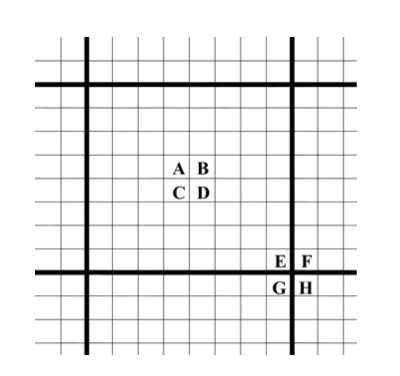
\includegraphics [width=4in]{block}

Using the $[A, B, C, D, E, F, G, H]$, noted above the \eqref{eq1} and
\eqref{eq2} are calculated
for every $8 \ \times \ 8$ block in the image.

\begin{align}
   Z'(i,j)=\abs{A-B-C+D}\label{eq1}\\
   Z''(i,j)=\abs{E-F-G+H}\label{eq2}
\end{align}

The values are then put into a normalized histogram, if the center values,
Z', histogram looks the same as the edge values Z'', histogram; then
the image was jpeg compressed.


\begin{verbatim}
im1=imread('Assignment4Files/blockArtifacts1.tif');
k1=blockDetect(im1);

im2=imread('Assignment4Files/blockArtifacts2.tif');
k1=blockDetect(im2);

im3=imread('Assignment4Files/blockArtifacts3.tif');
k1=blockDetect(im2);

type('blockDetect.m')
\end{verbatim}

        \color{lightgray} \begin{verbatim}

The strength of the blocking fingerprint is 5.842621e-01.
So the image was JPEG compressed 

The strength of the blocking fingerprint is 5.410334e-01.
So the image was JPEG compressed 

The strength of the blocking fingerprint is 5.410334e-01.
So the image was JPEG compressed 

function [ k ] = blockDetect( im )
%blockDetect implements the Fan and de Quieroz?s JPEG blocking artifact
    % detecting algorithm. inputs any image and output the k, blcoking 
    % strength value. 
    Zp=[]; 
    Zpp=[];
    [r,c]=size(im); 
    for i=1:8:r-8 % dont do the last 8x8 block in row or cols 
        for j=1:8:c-8
            grid=im(i:i+7,j:j+7); % grid plus one 
            A=grid(4,4); 
            B=grid(4,5); 
            C=grid(5,4); 
            D=grid(5,5); 
            Zp=[Zp, double(abs(A-B-C+D))]; 
            E=grid(8,8); 
            F=im(i+7,j+8); 
            G=im(i+8,j+7); 
            H=im(i+8,j+8); 
            Zpp=[Zpp, double(abs(E-F-G+H))]; 
        end 
    end 
    % 2)
    figure 
    HI=histogram(Zp,255); 
    HI.Normalization = 'probability'; 
    hold on 
    HII=histogram(Zpp,255); 
    HII.Normalization = 'probability'; 
    legend('Normalized center values','Normalized edge values')
    % 3)
    k=sum(abs(HI.Values-HII.Values)); 
    n=0.25; 
    % 4) 
    jpegDetect = (k>n); 
    fprintf('The strength of the blocking fingerprint is %d.\n',k); 
    if jpegDetect==1
        fprintf('So the image was JPEG compressed \n')
    else
        fprintf('So the image was not JPEG compressed \n')
    end

end

\end{verbatim} \color{black}

As seen below the Z' and Z'', histograms look very different. Also
the error of the two histograms was taken, called the blocking fingerprint.
The blocking fingerprint was then compared to a threshold of
0.25 to see if jpeg compression was detected.
    
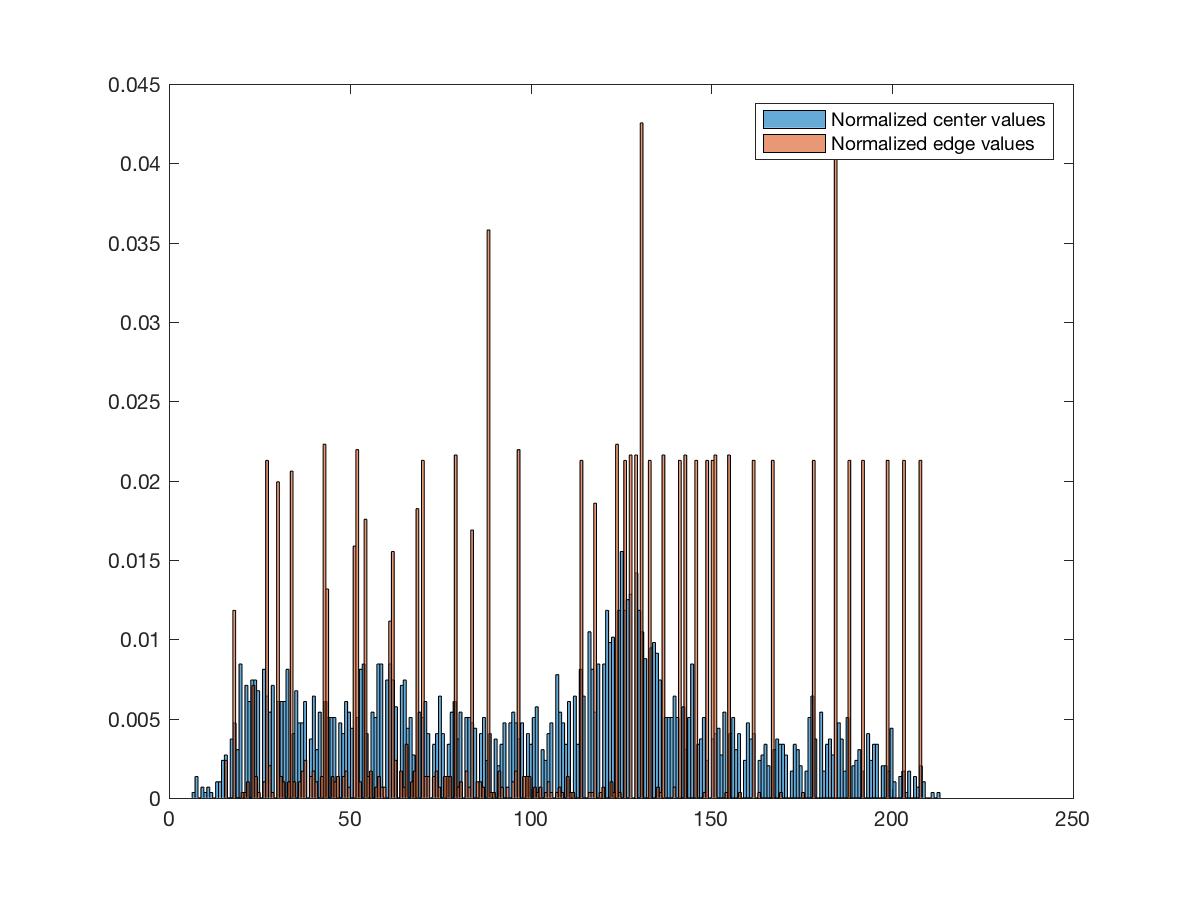
\includegraphics [width=3.5in]{lab4_01.eps}

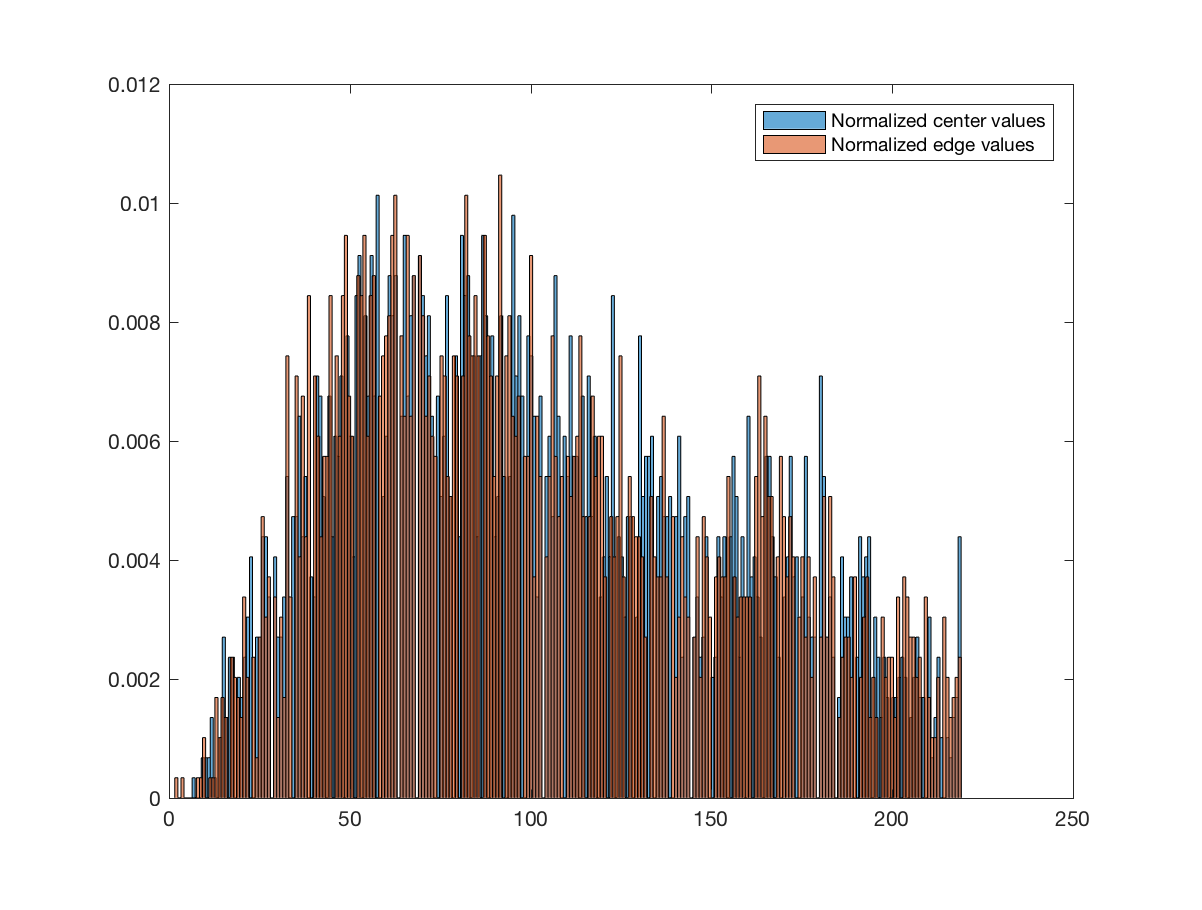
\includegraphics [width=3.5in]{lab4_02.eps}

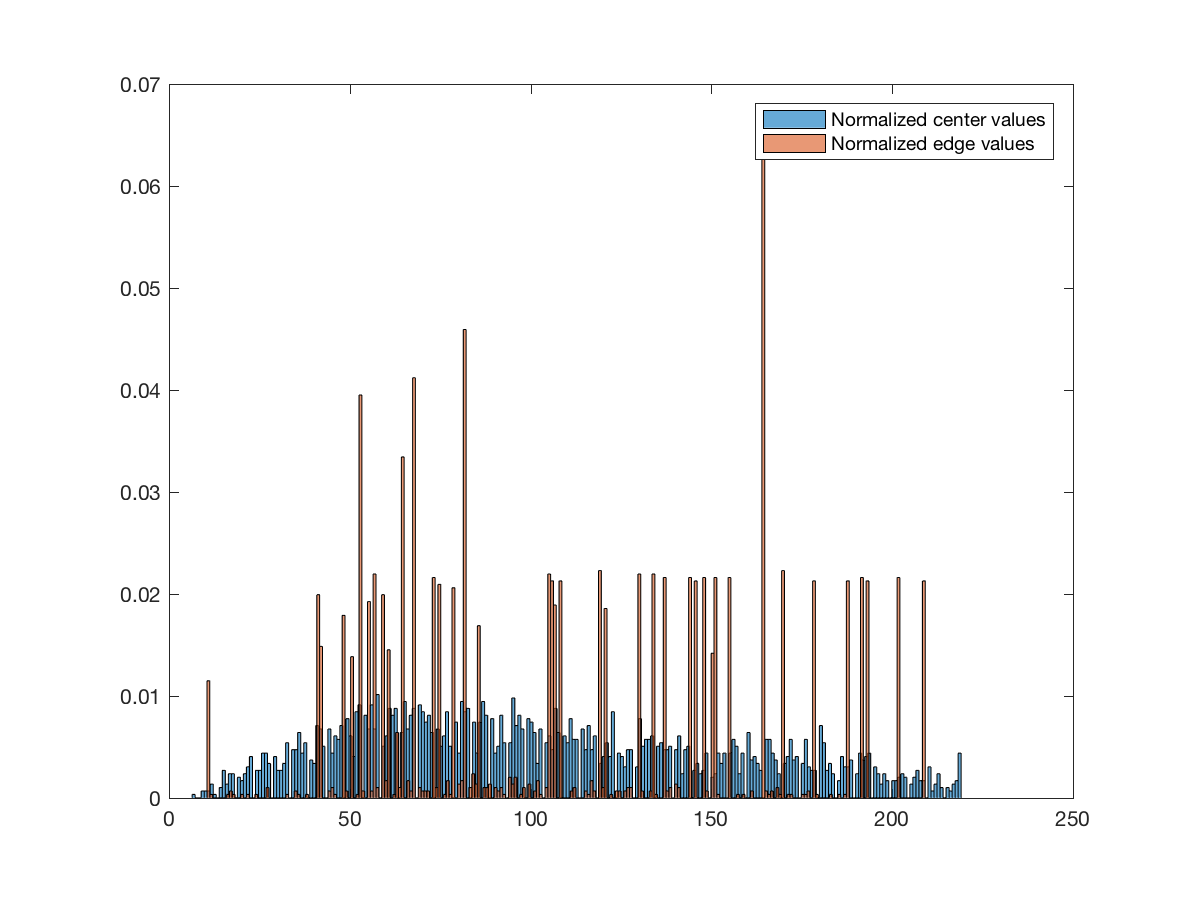
\includegraphics [width=3.5in]{lab4_03.eps}



\end{document}
    
